\begin{figure*}
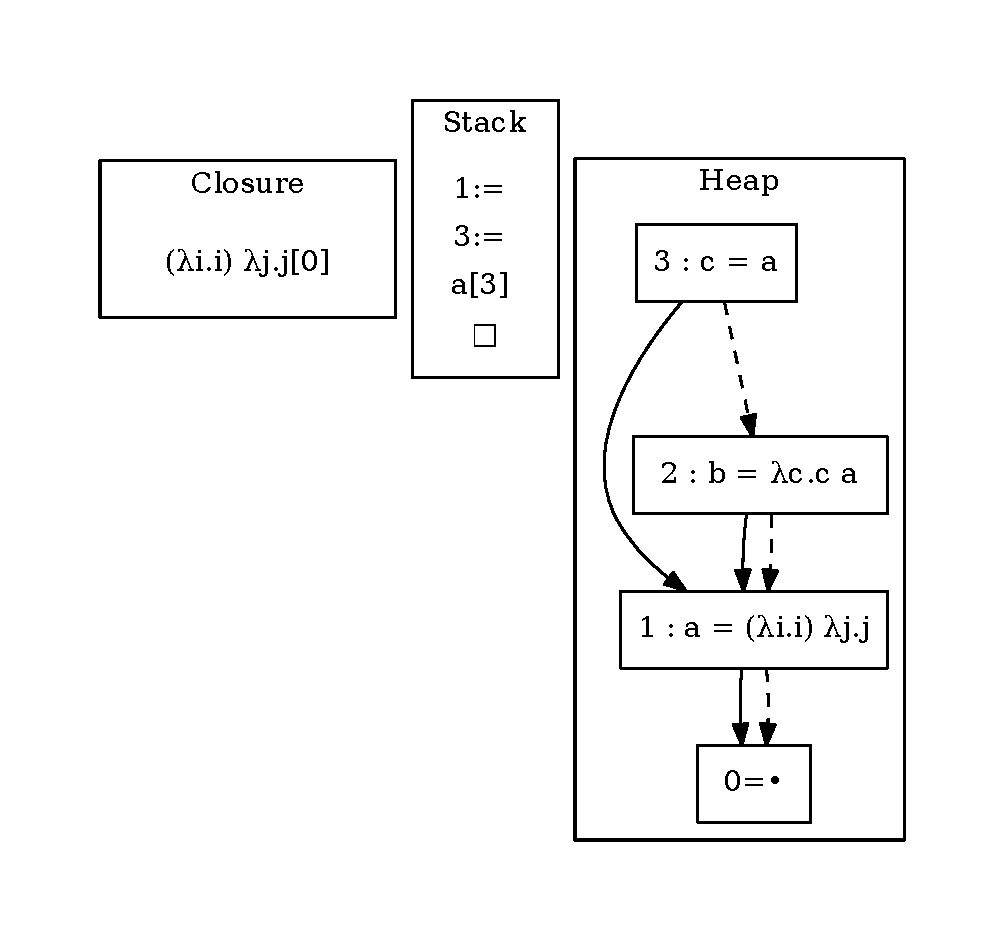
\includegraphics[width=\linewidth/3]{figures/12.pdf}
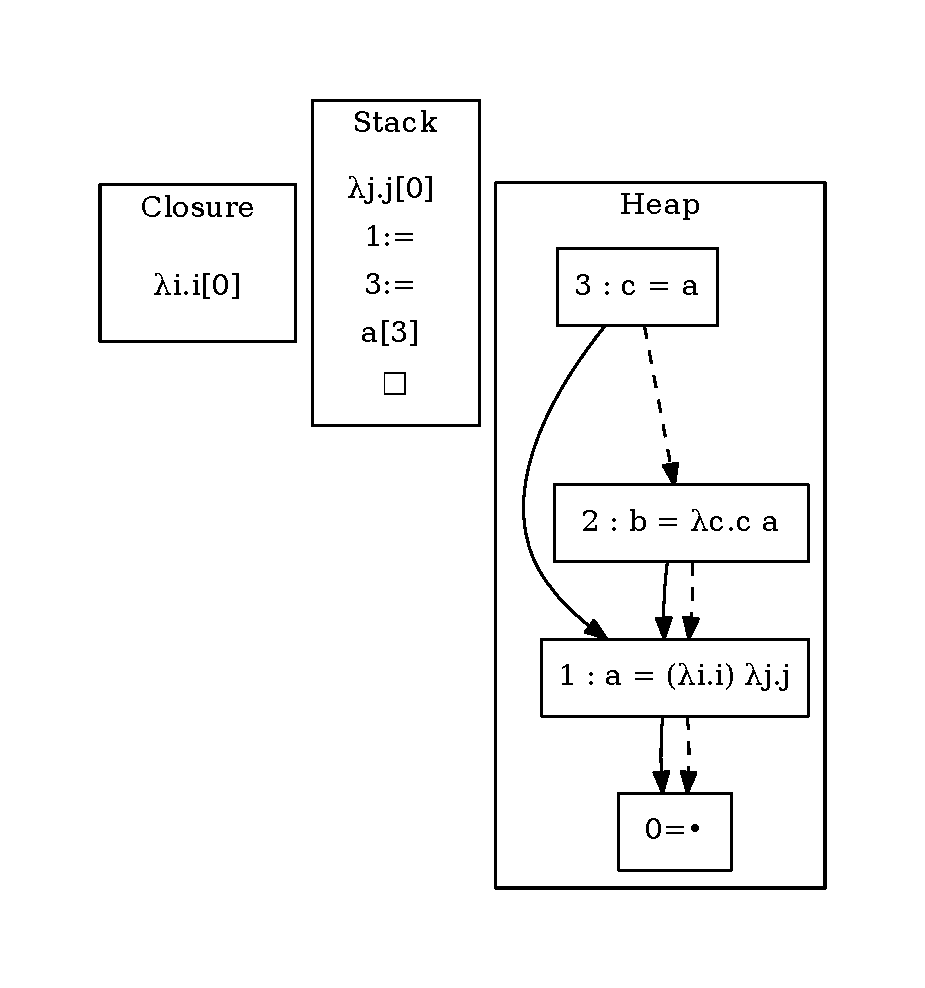
\includegraphics[width=\linewidth/3]{figures/13.pdf}
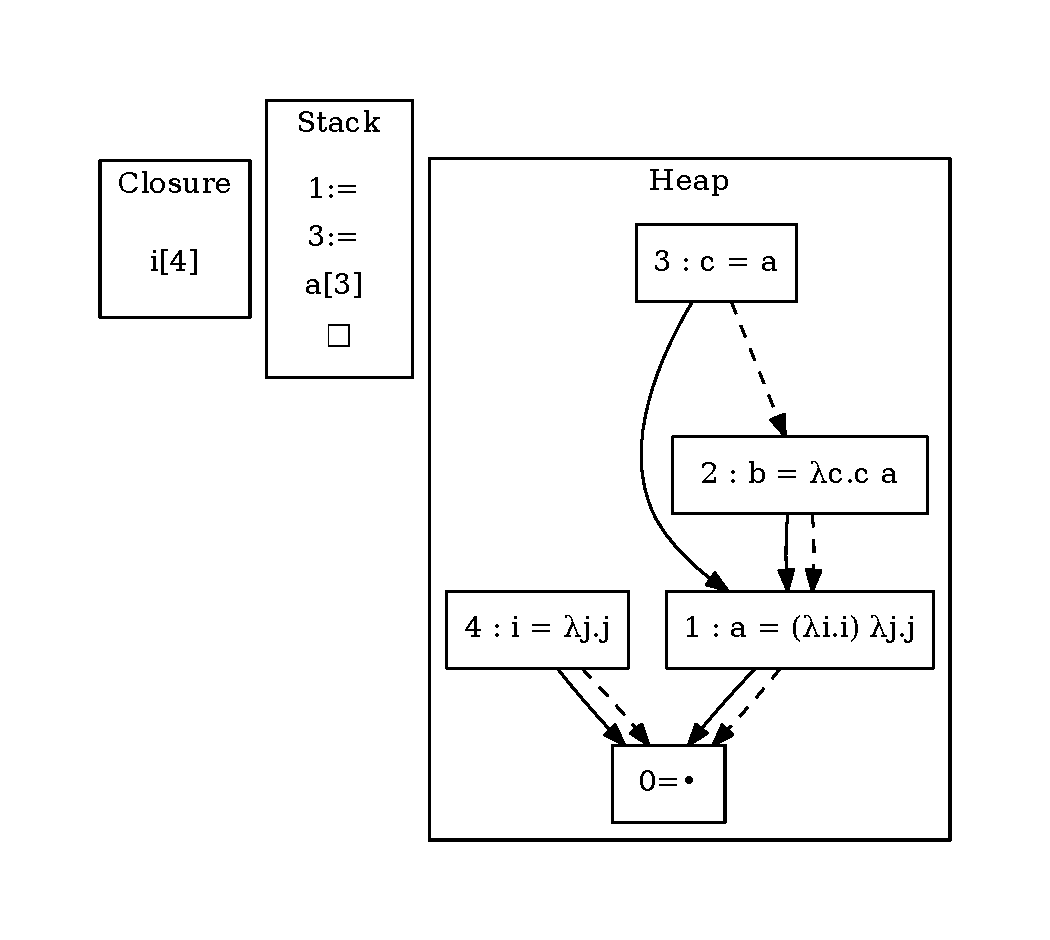
\includegraphics[width=\linewidth/3]{figures/14.pdf}
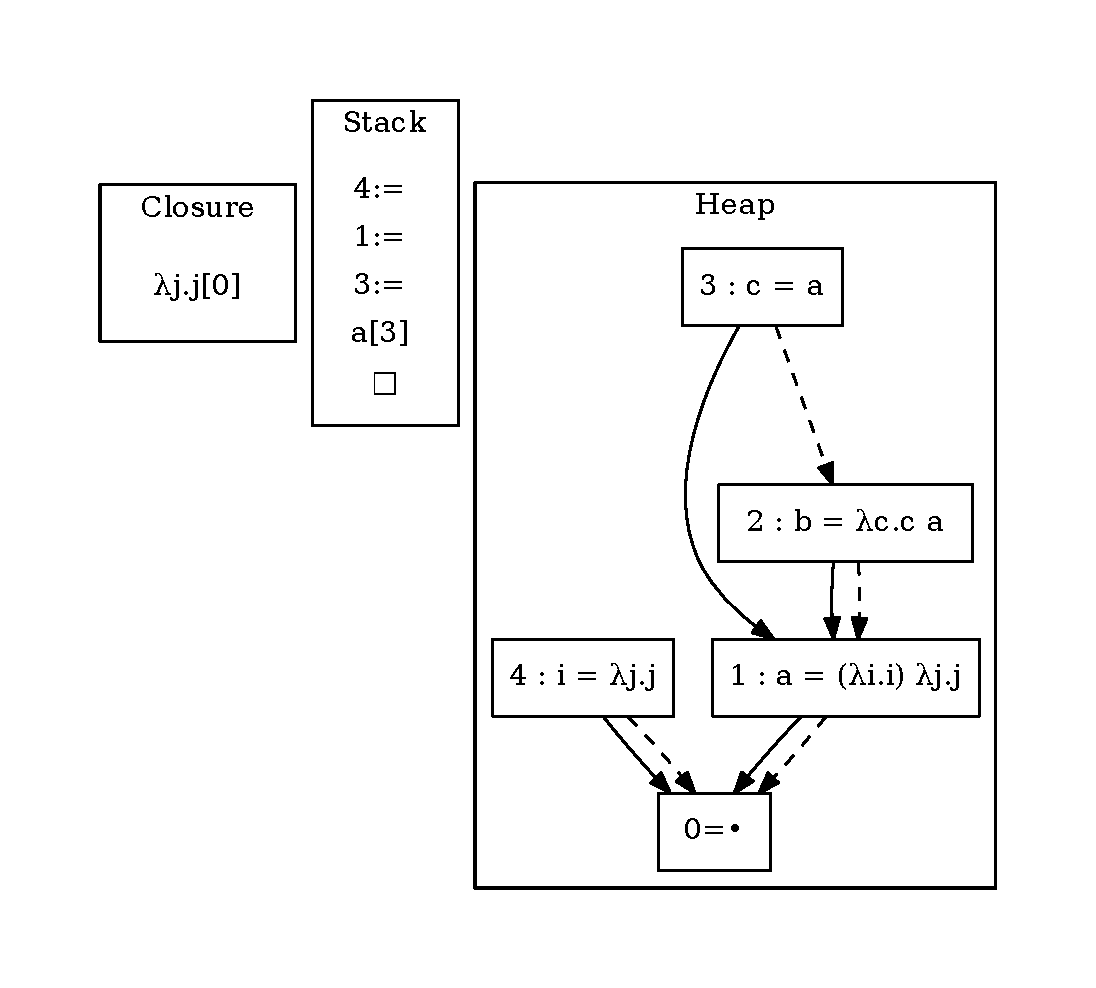
\includegraphics[width=\linewidth/3]{figures/15.pdf}
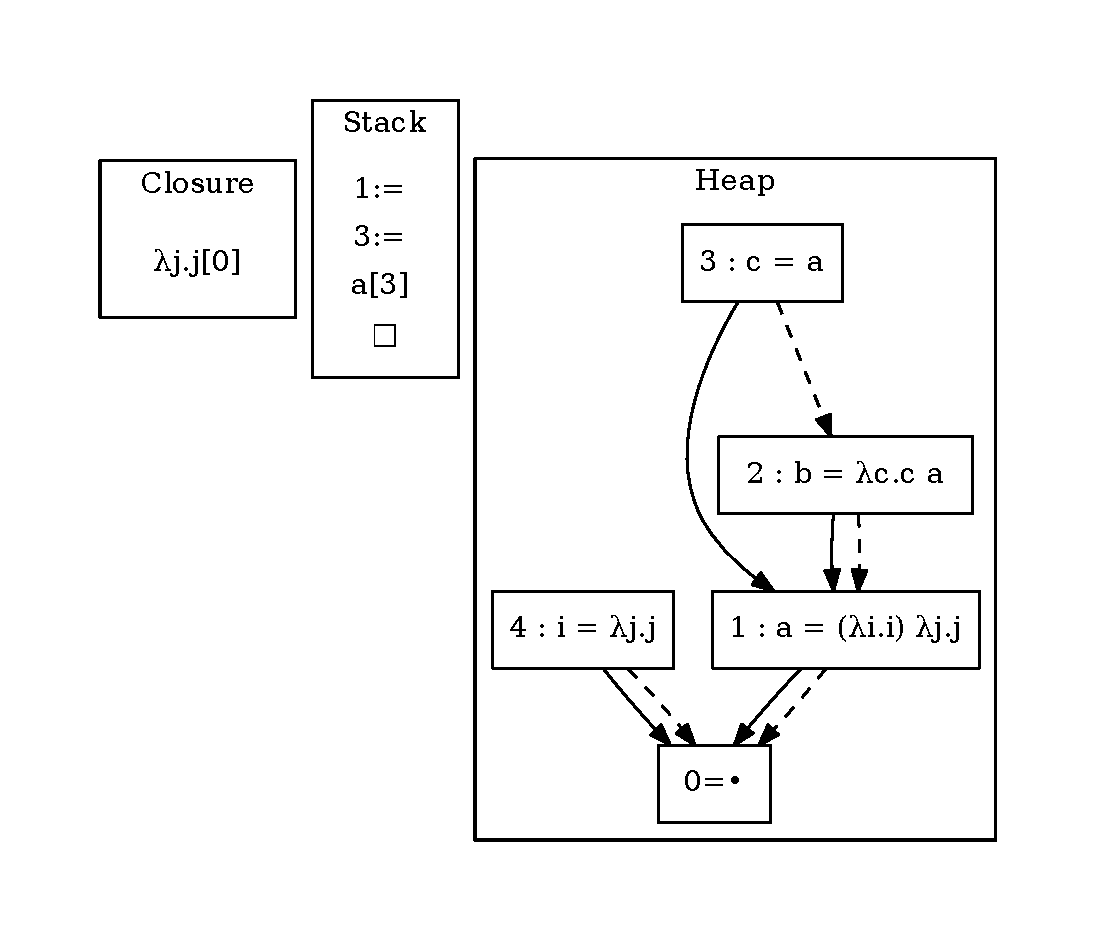
\includegraphics[width=\linewidth/3]{figures/16.pdf}
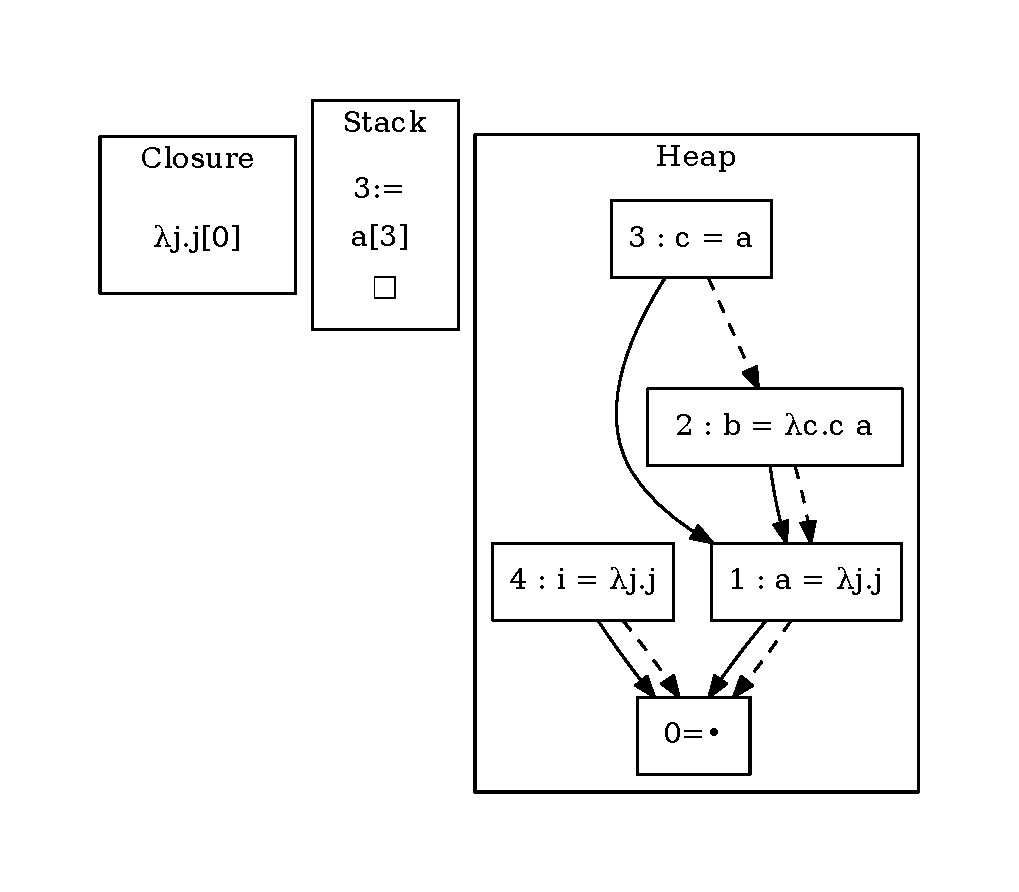
\includegraphics[width=\linewidth/3]{figures/17.pdf}
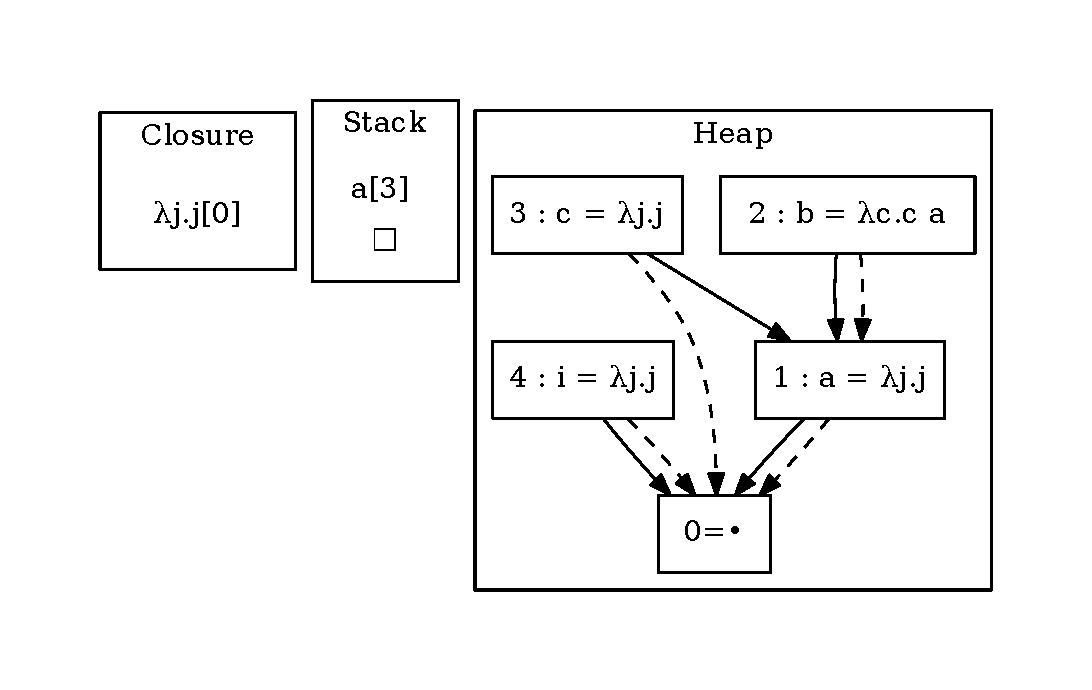
\includegraphics[width=\linewidth/3]{figures/18.pdf}
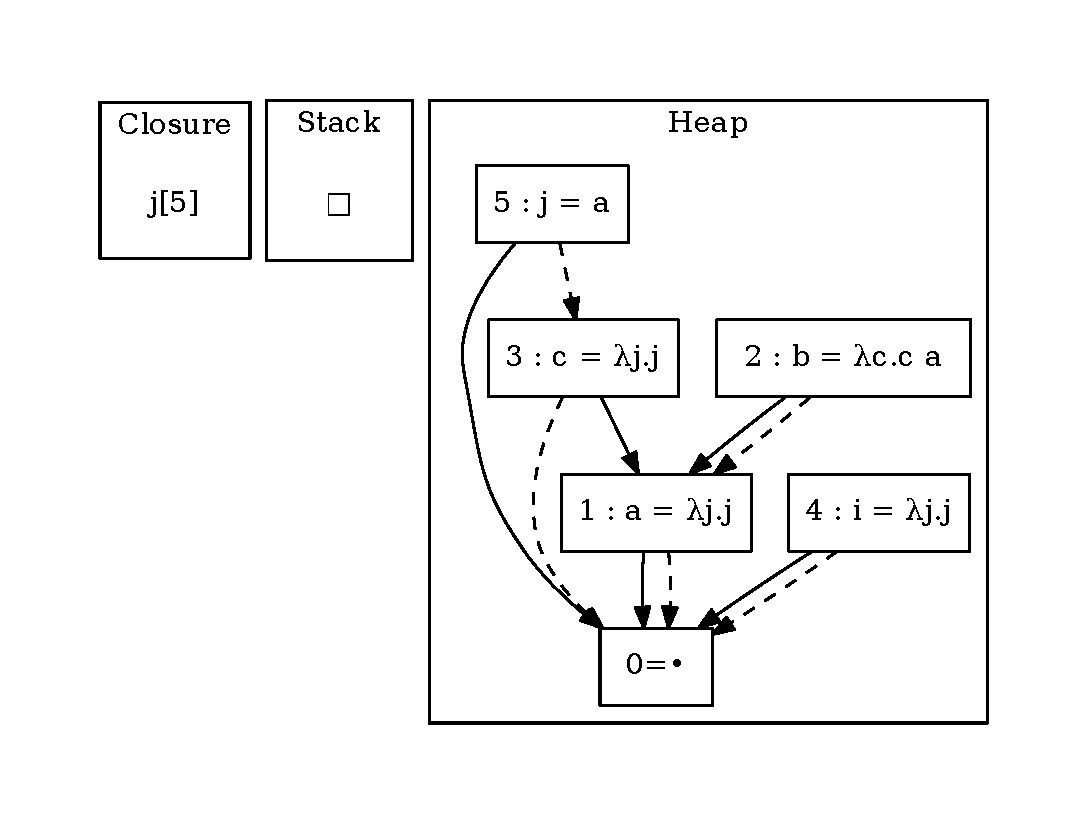
\includegraphics[width=\linewidth/3]{figures/19.pdf}
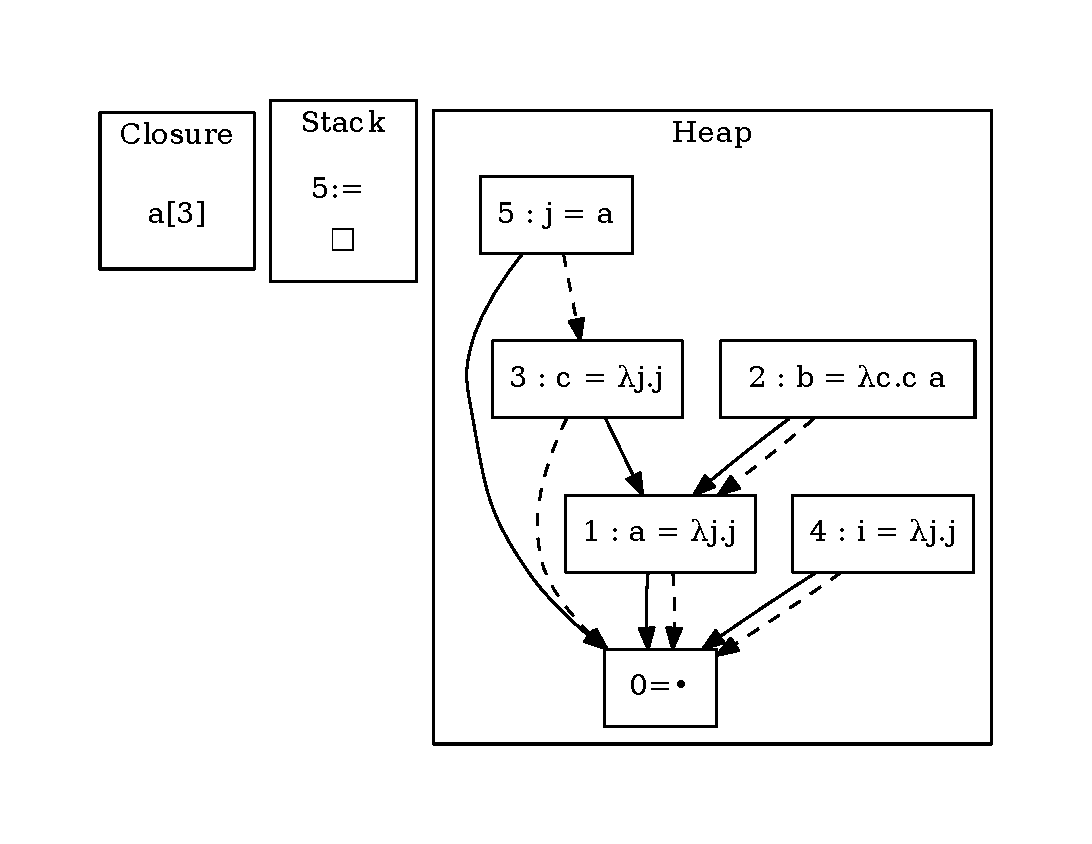
\includegraphics[width=\linewidth/3]{figures/20.pdf}
\caption{An example sequence of machine states during the evaluation of the term
$(\lambda a.(\lambda b.b \; a) (\lambda c.c
\; a)) ((\lambda i.i) (\lambda j.j))$. Order is left to right, top to bottom.
The free heap location $f$ is left out to save space. Dotted lines denote
the pointer for the closure's environment at a cell, and solid lines denote the
environment continuation. For example, in the first state, the environment
defined at location 3 corresponds to $c = a \cdot a = (\lambda i.i) \lambda j.j \cdot
\bullet$ in the $K$ machine's environment definition.  We see the App rule in
action in the transition from the first state to the second, which pushes the
argument term with the current environment onto the stack. The Lam rule is
expressed in the transition between the second and third states, where an
argument is popped and put in a fresh heap location. We see the update rule in
effect in a number of transitions, but most usefully in the transition from the
fifth to the sixth state, where $a=(\lambda i.i) \lambda j.j$ gets updated with
$\lambda j.j$. The Var rule transitions the third state to the fourth, where we
enter the closure $\lambda j.j[0]$.} \label{fig:states}
\end{figure*}
